\chapter{Implementation} \label{sec:implementation}

All development of the methods detailed in this section was done using Python.

\section{System diagram}

Figure \ref{fig:system} can help the reader to gain understanding how each of the materials and methods used as described in Section \ref{sec:mm} fit together.

\begin{figure}[h!]
    \centering
    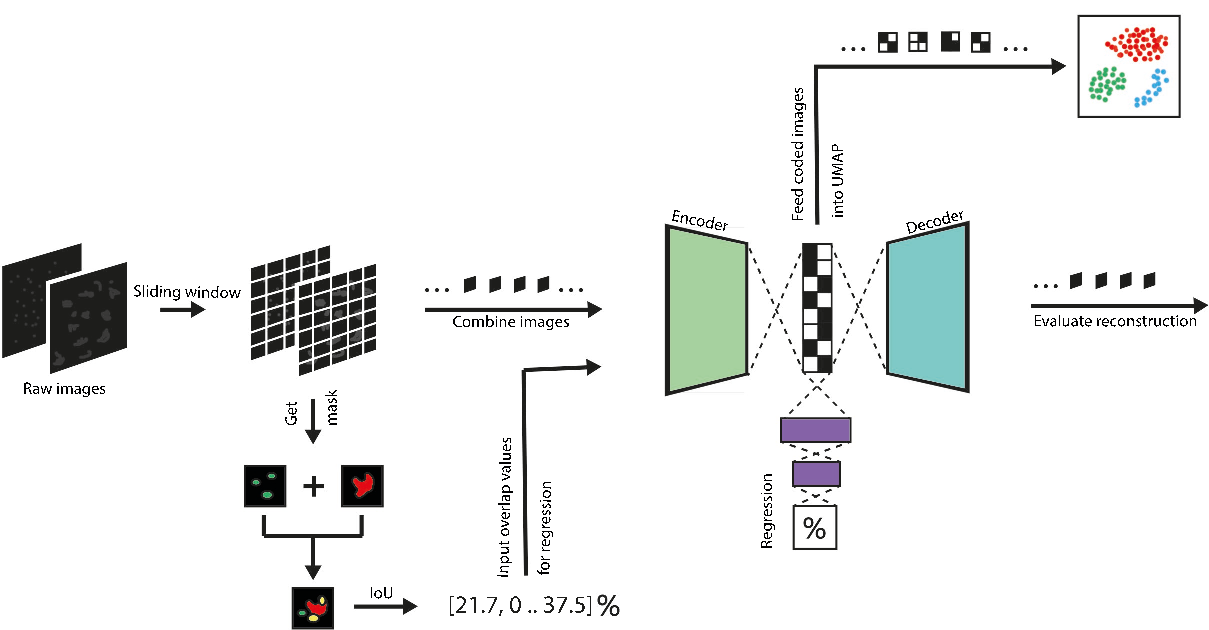
\includegraphics[width=\textwidth]{dissertation/figures/system_diagram.pdf}
    \caption{[TO ANNOTATE] System diagram showing how each image will be decomposed and analysed. The images will be transformed into smaller patches, from which we can gain overlap labels. On one hand, the smaller images will be fed into an autoencoder to accomplish dimensionality reduction and evaluate the success of projection of this smaller data in a two-dimensional plane. On the other hand, the smaller images will be fed in a regression model with the overlap labels in order to train a deep neural network for a regression task.}
    \label{fig:system}
\end{figure}

\section{Pre-processing}

Pre-processing steps are best illustrated through a diagram as shown in Figure \ref{fig:preprocessing}.

\begin{figure}[h]
    \centering
    \missingfigure[]{Figure showing pre-processing steps: raw images -> gridded images: 1. remove noise and normalise 2. obtain overlaps 3. combine images}
    \caption{Caption}
    \label{fig:preprocessing}
\end{figure}

Images were processed with a sliding window of size 192x192 as we wanted a window that was large enough to contain a few cells but also wanted to make it smaller to be able to reduce individual image dimensions further. A sliding window of 192x192 yielded 100 patches as our images were originally of size 2048x2048.

[further explanations?]

\section{Image segmentation}

Performing cell segmentation from grayscale microscope images of cells has been researched and is necessary when the cells to be studied in an image have not been separately labelled in one way or another. In our case, cell segmentation does not need to be applied as the images of T-cells and dendritic cells have been captured separately through fluorescent dyes. Instead, we are interested in using segmentation techniques to obtain the mask of each type of immune cell for the purposes of background correction and interaction quantisation, as explained in Section \ref{sec:segmentation}.

As our dataset pre-separated the type of immune cells and the cells were bright blobs on a background, we hoped that obtaining masks from each image would be straightforward. This section describes the methods we explored for this task. Both k-means and thresholding methods yielded good results and their specifics are detailed below.

\subsection{\textit{k}-means colour clustering}

k-means has been shown to perform well on image segmentation by quantising the number of colours in an image into \textit{k} clusters. Formally, k-means aims to partition data points in an array into \textit{k} sets such that the variance between points within clusters is minimised. In our case we wanted to use k-means to transform our black-and-white images of immune cells into bichrome images that we could use as masks. [The following pseudocode details the process of K-means.]

\begin{algorithm}[h]
    \DontPrintSemicolon
    \KwData{$I$, an array of pixel values making an image.\;
    $k$, the number of colours to partition the image's colour palette to.\;}
    \KwResult{A set of $k$ clusters.}
    \Begin{
        Initialise $k$ objects picked from $I$\;
        \While{clusters are still changing}
        {
           Assign each item $i$ in $I$ to the cluster with closest mean value\;
           Recompute the mean of each cluster\;
        }
    }

\caption{Pseudocode for the k-means algorithm applied to image segmentation.}
\label{alg:kmeans}
\end{algorithm}

k-means clustering is conveniently offered by multiple libraries in Python. We looked at both scikit-learn's and OpenCV's k-means. scikit-learn is a general library  for machine learning tools, while OpenCV is a more specialised library built for Computer Vision purposes. Both their k-means functions are straightforward to initialise and use. Their performance was benchmarked in order to select the best one. The table below reports times for k-means with \textit{k}=2, 10 iterations, and each of the random and optimised methods of initialising centroids.

\begin{table}[h]
\centering
\begin{tabular}{|l|l|l|}
\hline
\textbf{Initialisation} & \textbf{OpenCV} & \textbf{Scikit-learn} \\ \hline
Random                                   & \multicolumn{1}{r|}{18.9s}       & \multicolumn{1}{r|}{165s}              \\ \hline
k-means++                                & \multicolumn{1}{r|}{29.3s}       & \multicolumn{1}{r|}{139s}              \\ \hline
\end{tabular}

\caption{CPU times for OpenCV's and scikit-learn's k-means tool ran on 1,000 samples of 192x192 pixels with different methods of initialising centroids.  The computation was ran on a 2015 MacBook Pro with 2.7 GHz i5 core and 8 GB memory.}
\end{table}

As we can see OpenCV outperforms scikit-learn in all cases. OpenCV for Python is a wrapper library around the original OpenCV code built in C++, which gives it a boost in performance. OpenCV's k-means was thus selected. Initially, k-means centers were initialised randomly in development for the boost of performance. However, during validation it was found that this method of initialisation was yielding highly different results for the intersection-over-union metric at every run. Hence, some speed was traded for consistency and the kmeans++ center initialisation method was picked instead.

\subsection{Thresholding}

An alternative to k-means in the case of black-and-white images is thresholding. We decided to explore this option as it could have performance improvements compared to K-means.

Thresholding refers to the process of converting a grayscale image to a binary image of pixels. Pixels above a set threshold are set to 1, and the rest of the pixels below that threshold are set to 0. Thresholding depends on pixel distribution analysis. Usually, thresholding works well for images which have different peaks of pixel values in their distribution. We can then pick the value which seems to separate out the two peaks as our threshold. However, in the case of our images we had one visible peak of pixel values and could not identify a viable threshold from the histogram. Figure \ref{fig:thresholdhist} illustrates this.

\begin{figure}[h]
    \centering
    \begin{subfigure}{0.45\textwidth}
        \centering
        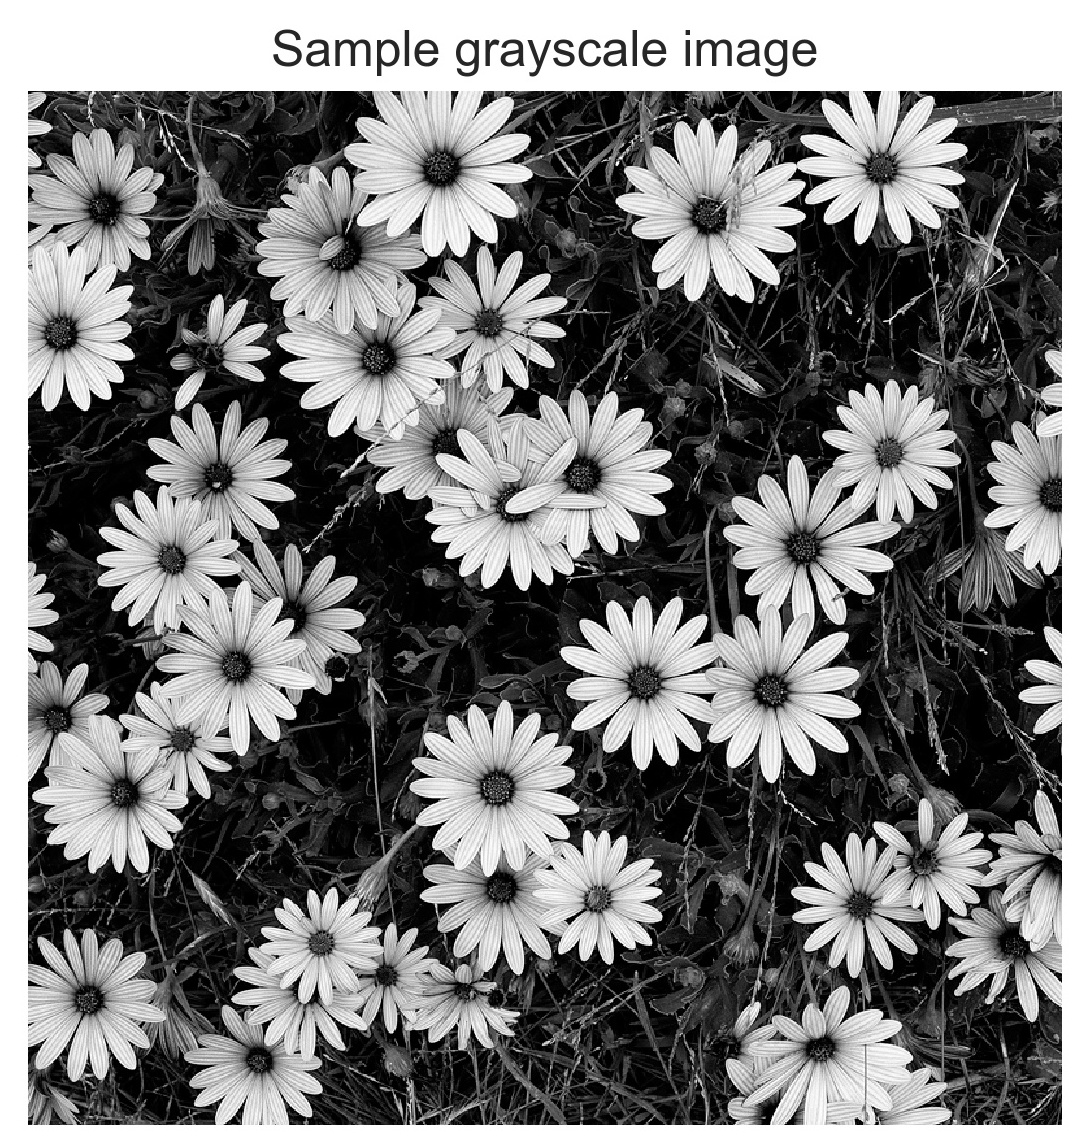
\includegraphics[width=.5\textwidth]{dissertation/figures/sample_grayscale.jpg}
    \end{subfigure}
    \begin{subfigure}{0.45\textwidth}
        \centering
        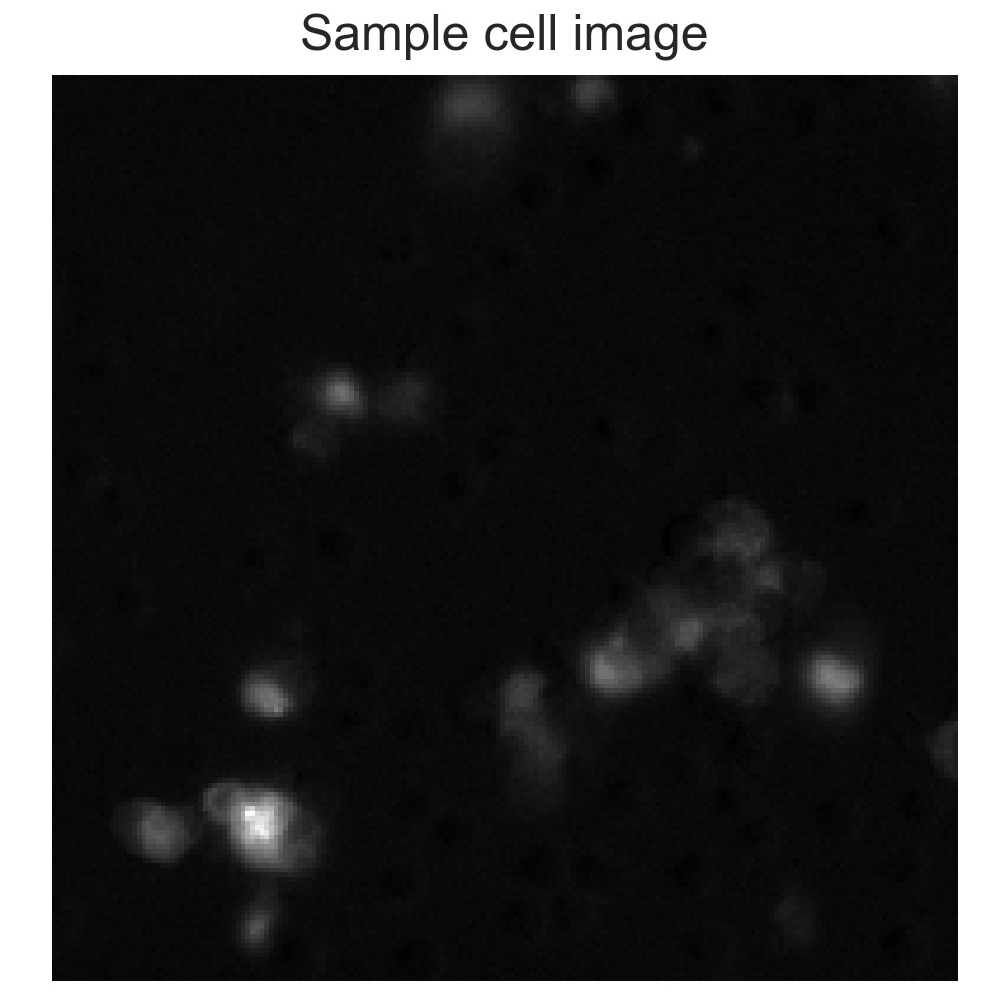
\includegraphics[width=.5\textwidth]{dissertation/figures/sample_cell.jpg}
    \end{subfigure}
    \begin{subfigure}{0.45\textwidth}
        \centering
        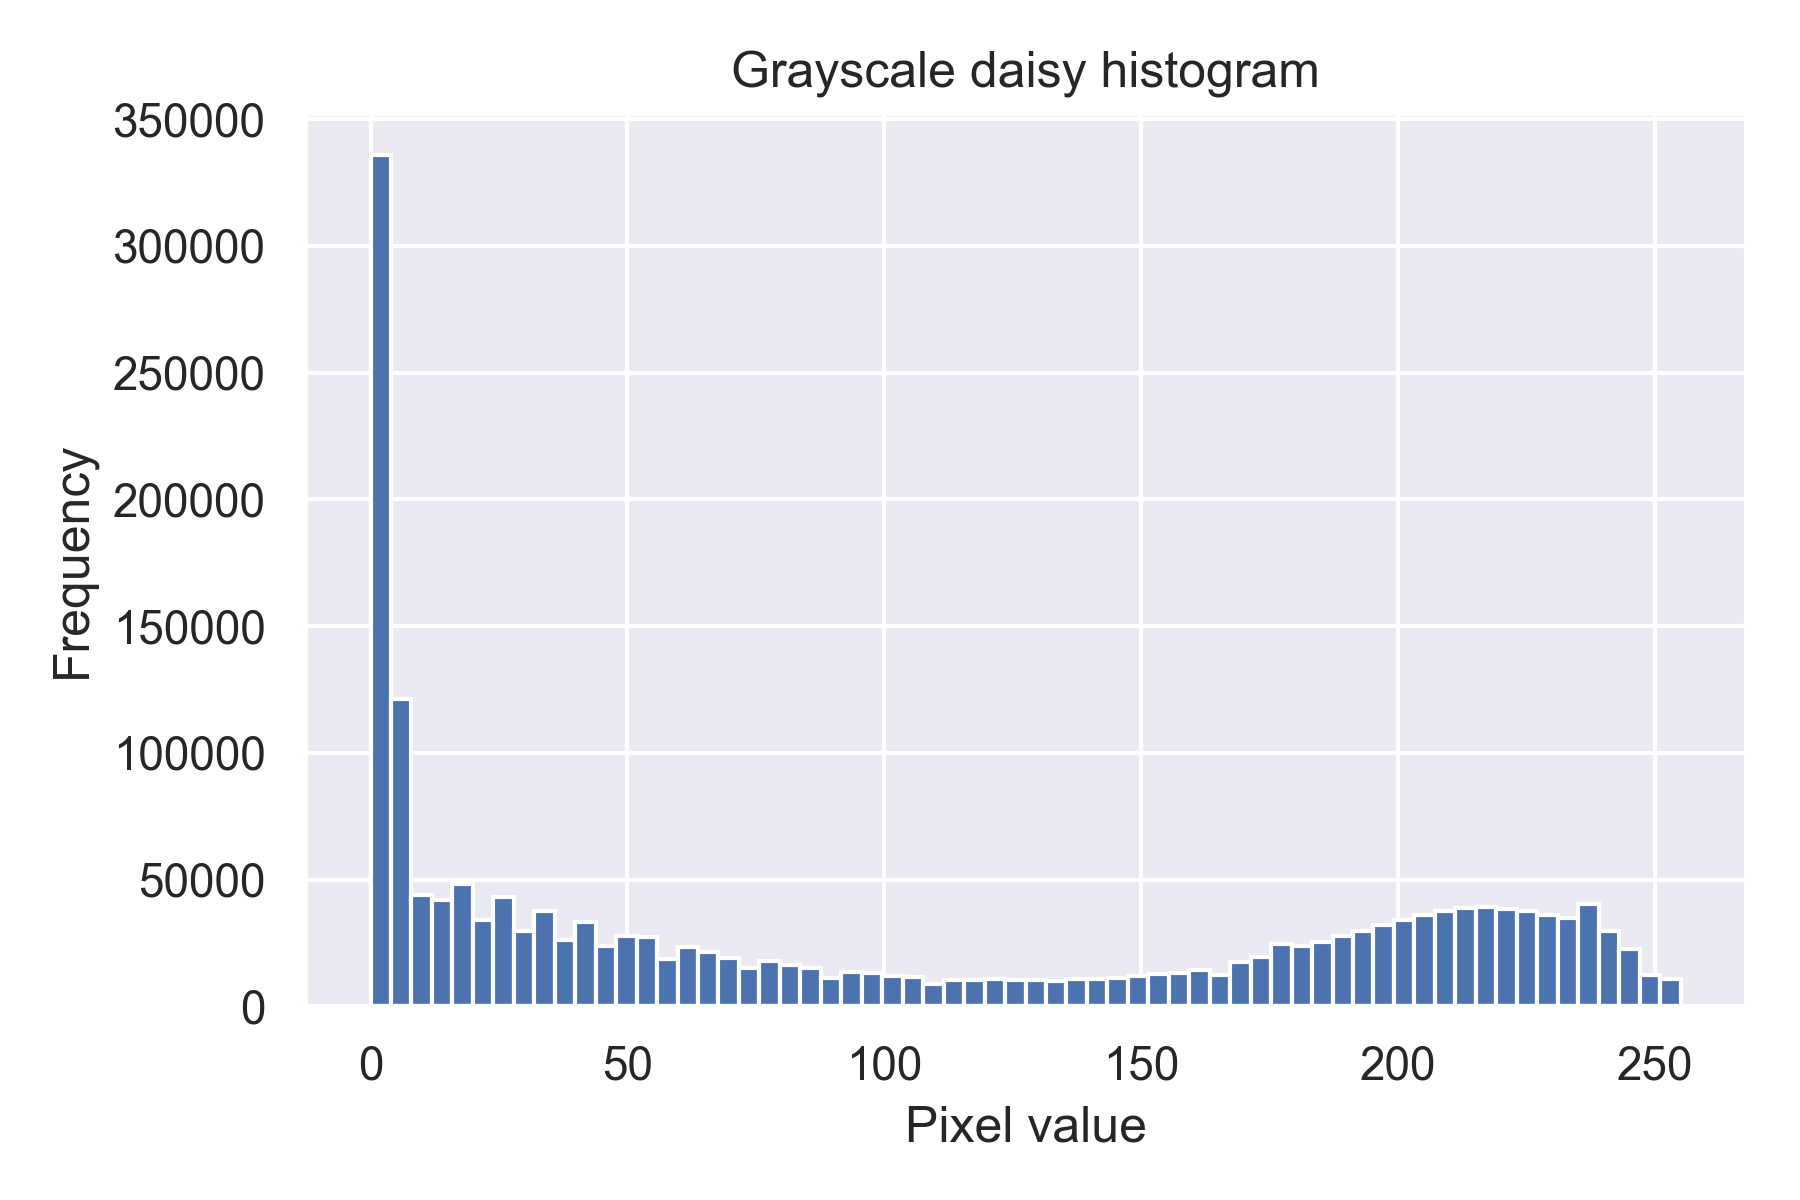
\includegraphics[width=.5\textwidth]{dissertation/figures/grayscale_histogram.png}
    \end{subfigure}
    \begin{subfigure}{0.5\textwidth}
        \centering
        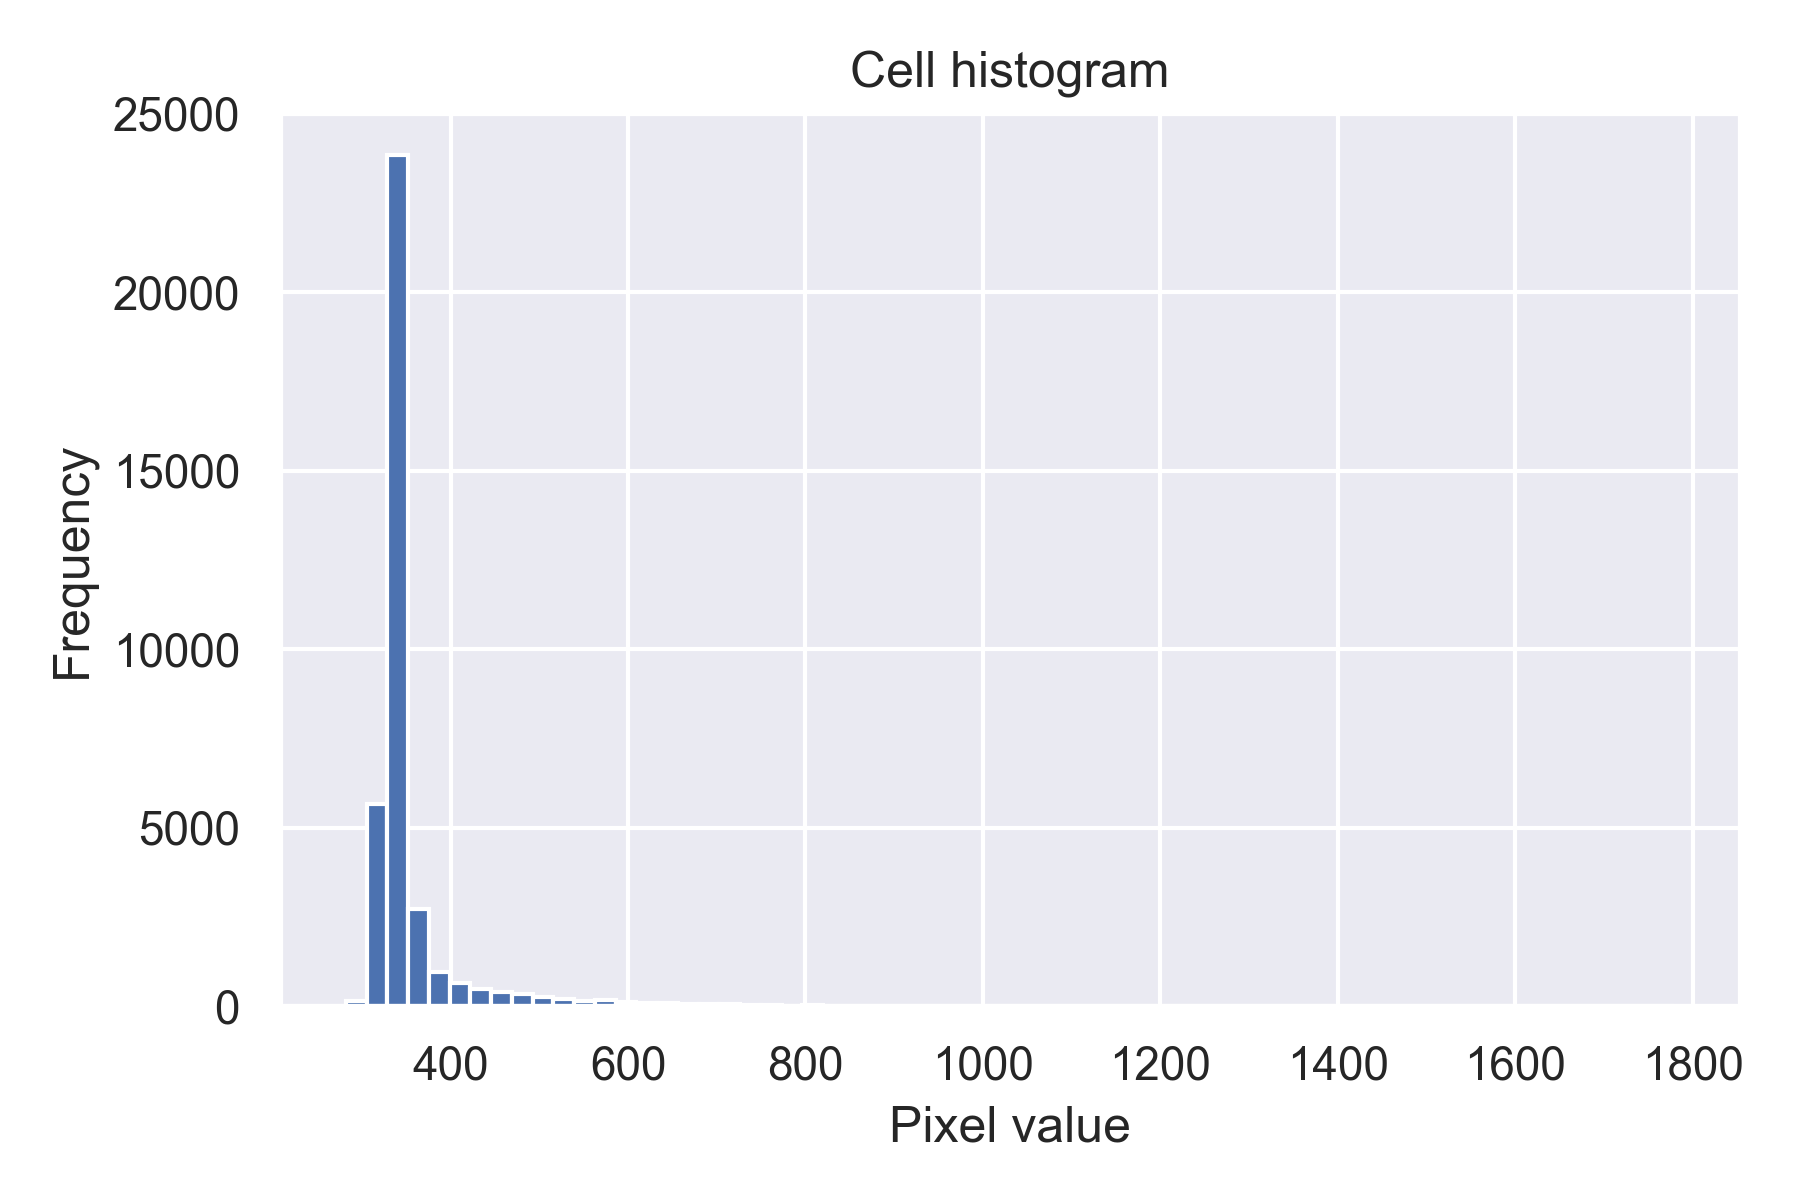
\includegraphics[width=.45\textwidth]{dissertation/figures/cell_histogram.png}
    \end{subfigure}
    \caption{Example images and their histogram. As we can see the grayscale image of lillies has two peaks of frequency, and we can see there is a separation between the peaks at a pixel value of around 110. The grayscale image of a cell has one peak, and there is a smaller frequency of pixel values past that peak, but we cannot identify a specific pixel value as a threshold from the histogram.}
    \label{fig:thresholdhist}
\end{figure}
As such, we had to find an alternative for finding a suitable threshold. First, we selected the mean pixel value as the threshold. This yielded acceptable results, however some noisy pixels still came through the mask (see Figure \ref{fig:thresholdmean}). To fix that problem, the threshold value was set as the sum of the mean pixel value and the standard deviation. This decision was based on the hypothesis that the noise level of an image with a flat structure can be estimated from its variation. Results were satisfactory, as shown in Figure \ref{fig:thresholdstd}.

\begin{figure}[h]
    \centering
    \begin{subfigure}[h!]{0.4\textwidth}
        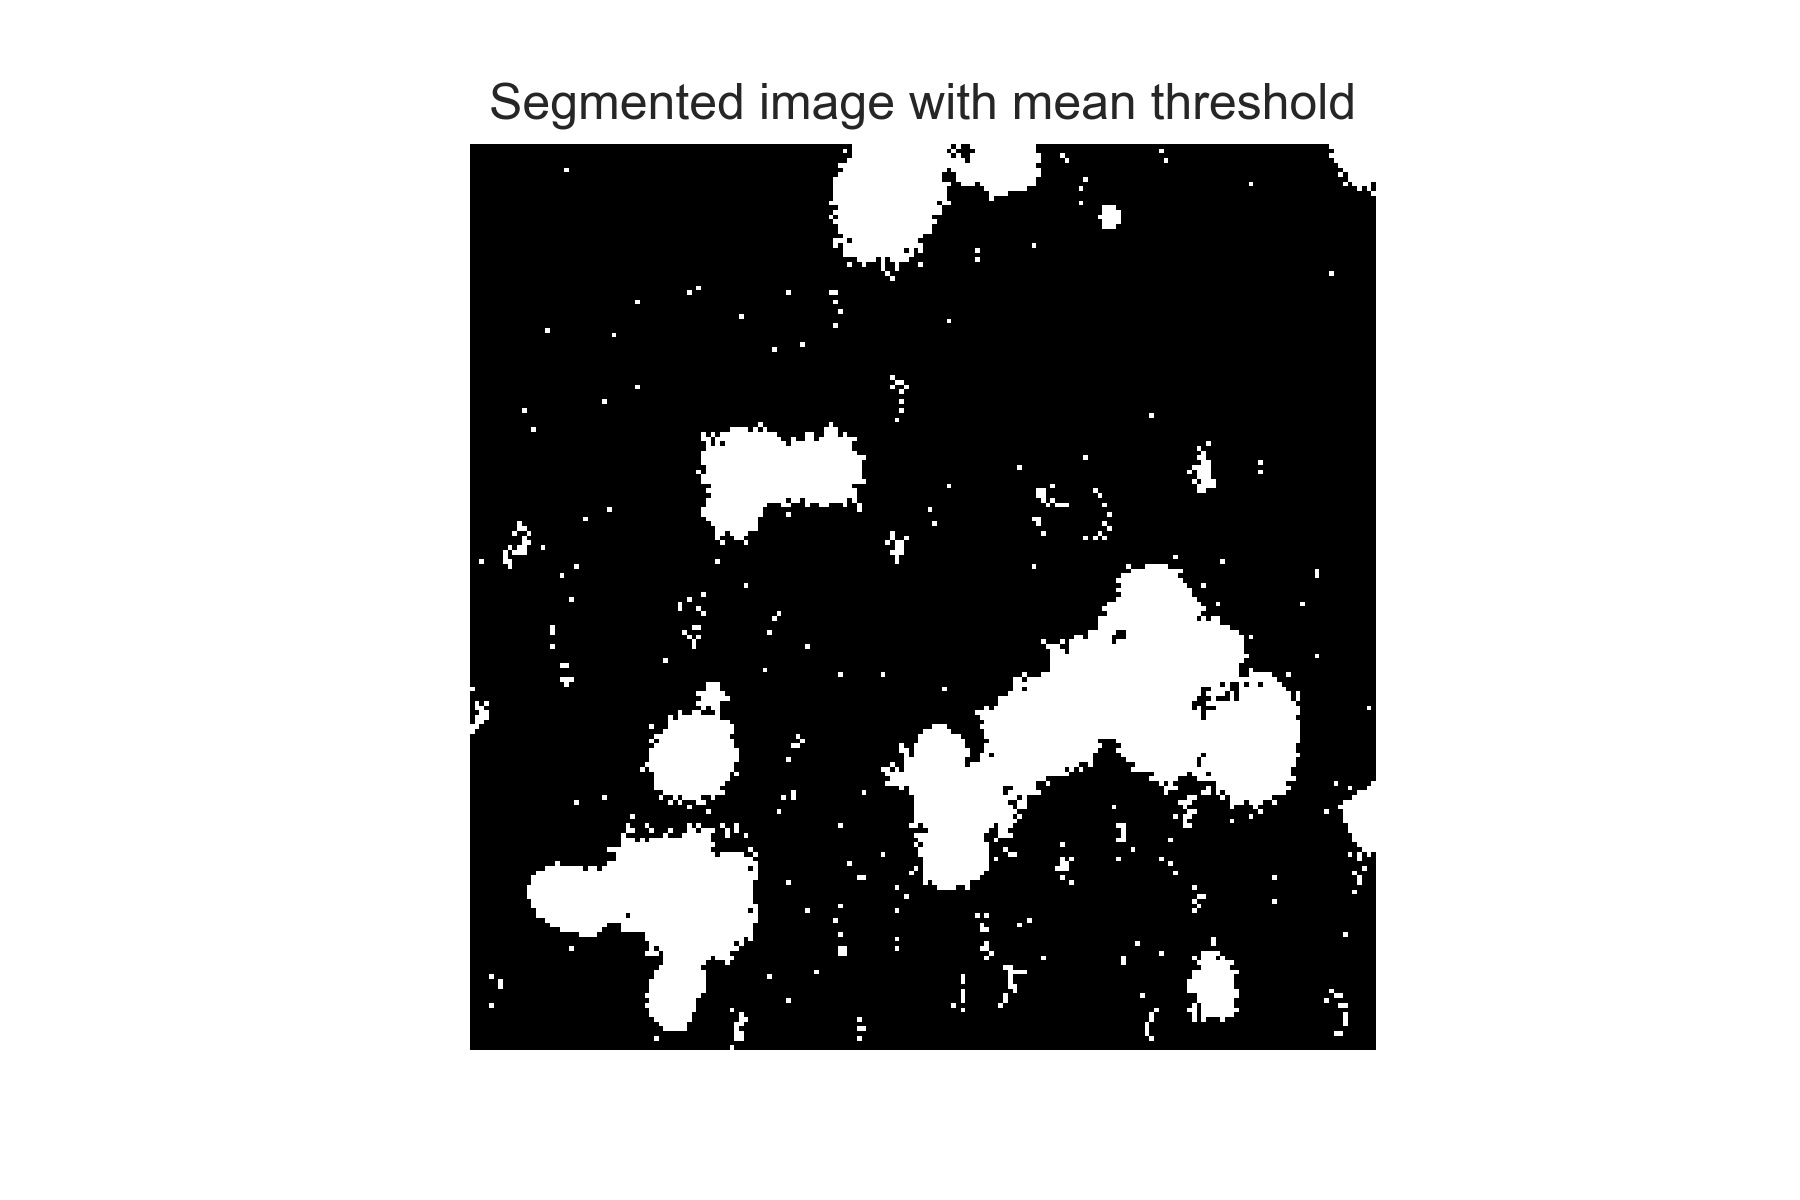
\includegraphics[width=\textwidth]{dissertation/figures/mean_threshold_cell.jpg}
        \caption{Threshold: mean pixel value}
        \label{fig:thresholdmean}
    \end{subfigure}
    \begin{subfigure}[h!]{0.4\textwidth}
        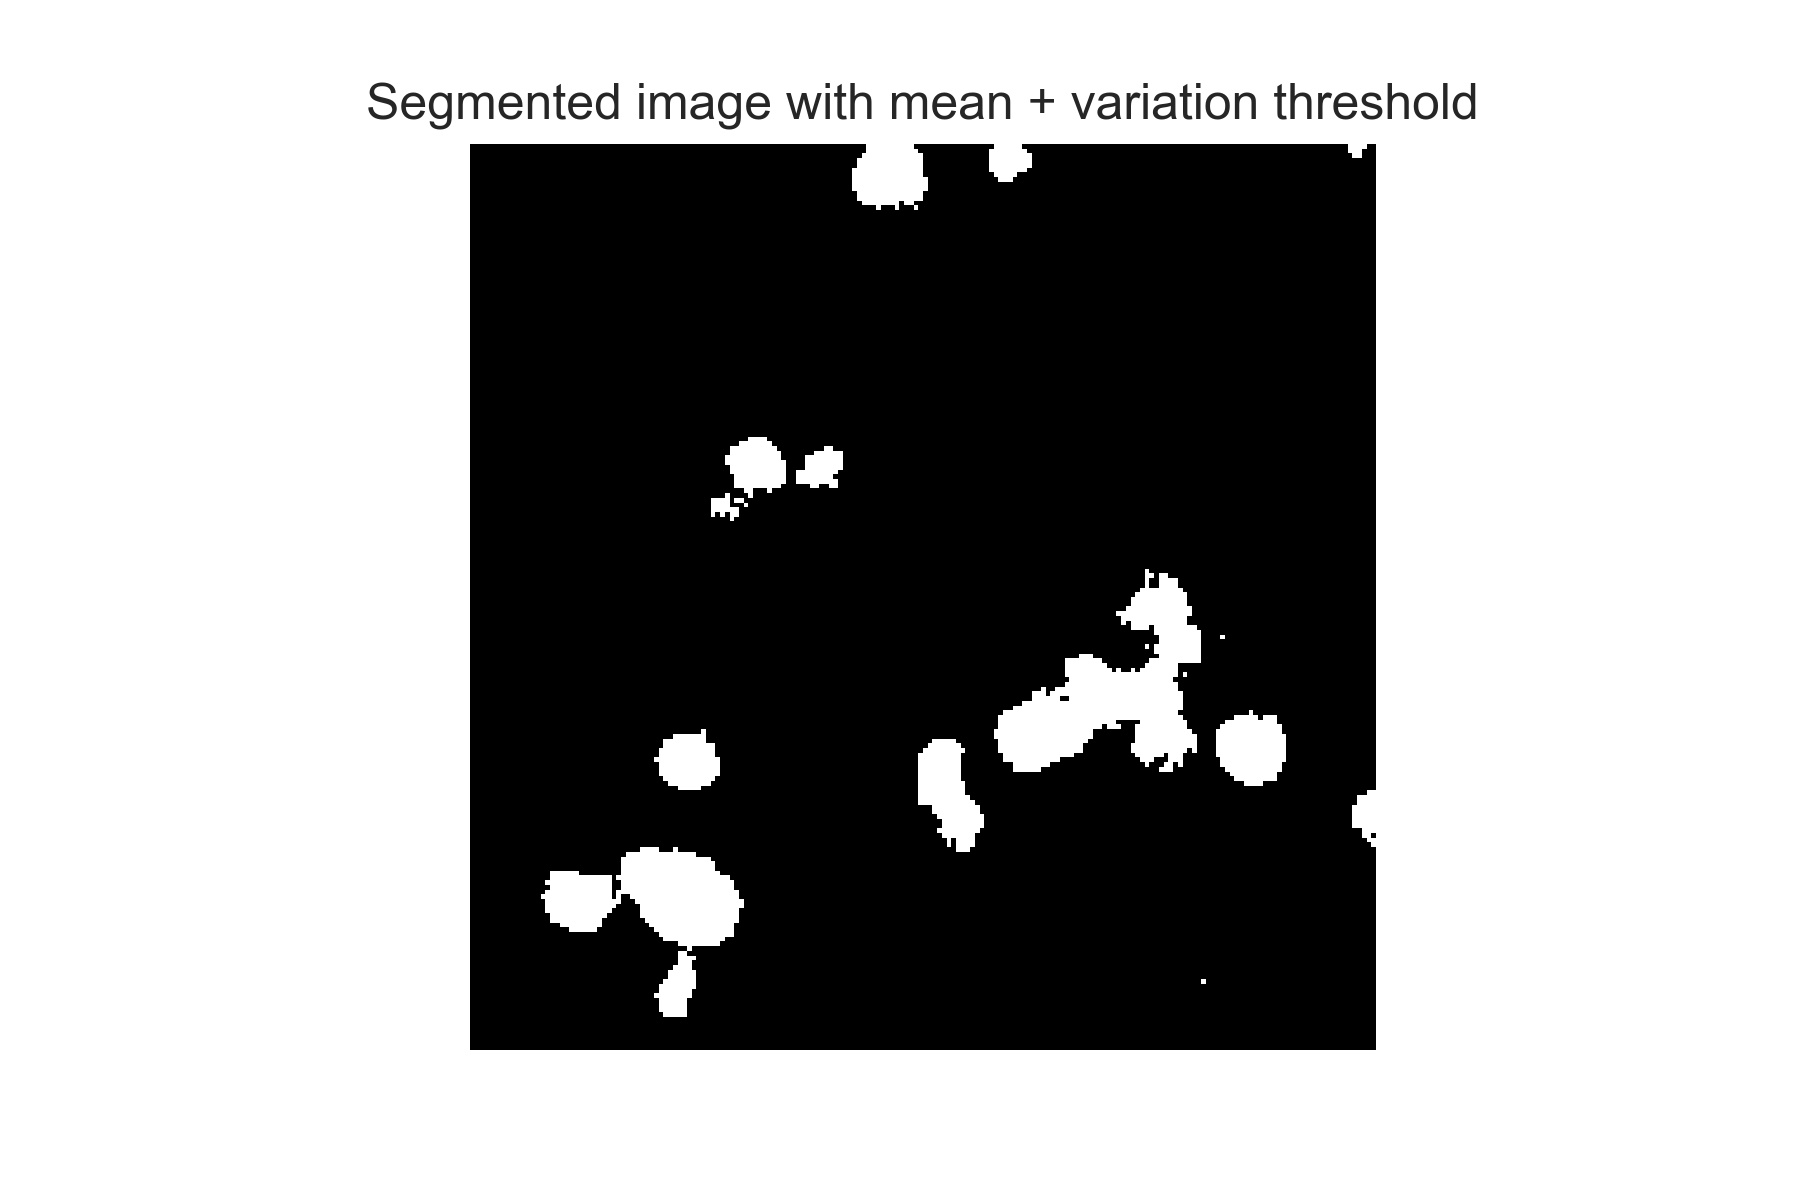
\includegraphics[width=\textwidth]{dissertation/figures/mean_std_threshold_cell.jpg}
        \caption{Threshold: mean + standard deviation}
        \label{fig:thresholdstd}
    \end{subfigure}
    \caption{Segmented images according to different threshold values.}
\end{figure}

Image segmentation through thresholding is also much faster than k-means, with 1,000 images being processed in [360 milliseconds] with the use of NumPy arrays. Nonetheless, masks yielded by k-means are more granular. Figure \ref{fig:maskdiff} shows the difference between the masks obtained through different methods.

\begin{figure}[h]
    \centering
    \missingfigure[]{Binary image showing the absolute difference between a mask obtained with k-means and one obtained with thresholding.}
    \caption{Binary image showing the absolute difference between a mask obtained with k-means and one obtained with thresholding.}
    \label{fig:maskdiff}
\end{figure}

\subsection{UNet}

[mention UNet findings here?]

\section{Autoencoder and regression models}

\subsection{Experimental setup}

As this is a research project based on using deep learning models, a large part of the research involved an iterative process of repetitively tweaking the deep learning models, training them, and evaluating them. Immunology experiments produce a lot of imaging data, and we wanted our models to perform well on unseen data. Moreover, not all datasets contained instances of all classes. We wanted our trained model to be able to deal with such datasets too. As such, we selected the full dataset containing instances for all classes for training our model (see Table \ref{table:datasets}). Part of it was set out for validation and testing. The other two selected datasets were used purely for testing. Table \ref{table:splits} reports the number of samples in each dataset.

\begin{table}[h]
\centering
\begin{tabular}{l|r|r|r}
\hline
\rowcolor[HTML]{EFEFEF}
Dataset       & Train  & Validation & Test   \\ \hline
Full & 16,490 & 2,910      & 10,000 \\
Dual   &        &            & 15,900 \\
DMSO          &        &            & 8,000  \\ \hline
\end{tabular}
\caption{Train-test-validation splits for selected datasets. Models are only to be trained on the full, balanced dataset. The validation set represents 15\% of the training set.}
\label{table:splits}
\end{table}

All deep learning development was done using Keras\footnote{https://keras.io} for Python on a Tensorflow backend. Training was carried out on Google Colaboratory notebooks\footnote{https://colab.research.google.com/} to be able to accelerate computations with Google's GPUs.

While training, we used Keras's callbacks feature to monitor the model's validation loss and change training parameters accordingly. The model would reduce its learning rate by a factor of 0.2 if no improvements in the validation loss were seen over 3 epochs, and it would completely stop training if no improvements were witnessed in validation loss over 5 epochs. Training was usually ran with a batch size of 64 over 40 epochs.

\subsection{Convolutional autoencoder}

The main model to be developed was a convolutional autoencoder. The autoencoder was built for two purposes: obtaining a smaller \textit{code} representing each of the images to be fed into high-dimensional visualisation algorithms, and to be the building block for a deep regression model.

An autoencoder follows a symmetrical structure of reduction and expansion operations. The reduction operations represent the encoding part of our model, and the expansion operations represent the decoding part of our model. In order for the autoencoder input to be reduced and then reconstructed to the same number of input dimensions, we need the two sets of operations to follow the same pattern and use the same number of parameters. Figure \ref{fig:symmstruc} illustrates the symmetrical structure of an autoencoder, and shows the core layers of a convolutional autoencoder: convolution layers combined with activation functions, and pooling/upsampling layers.

\begin{figure}[h]
    \centering
    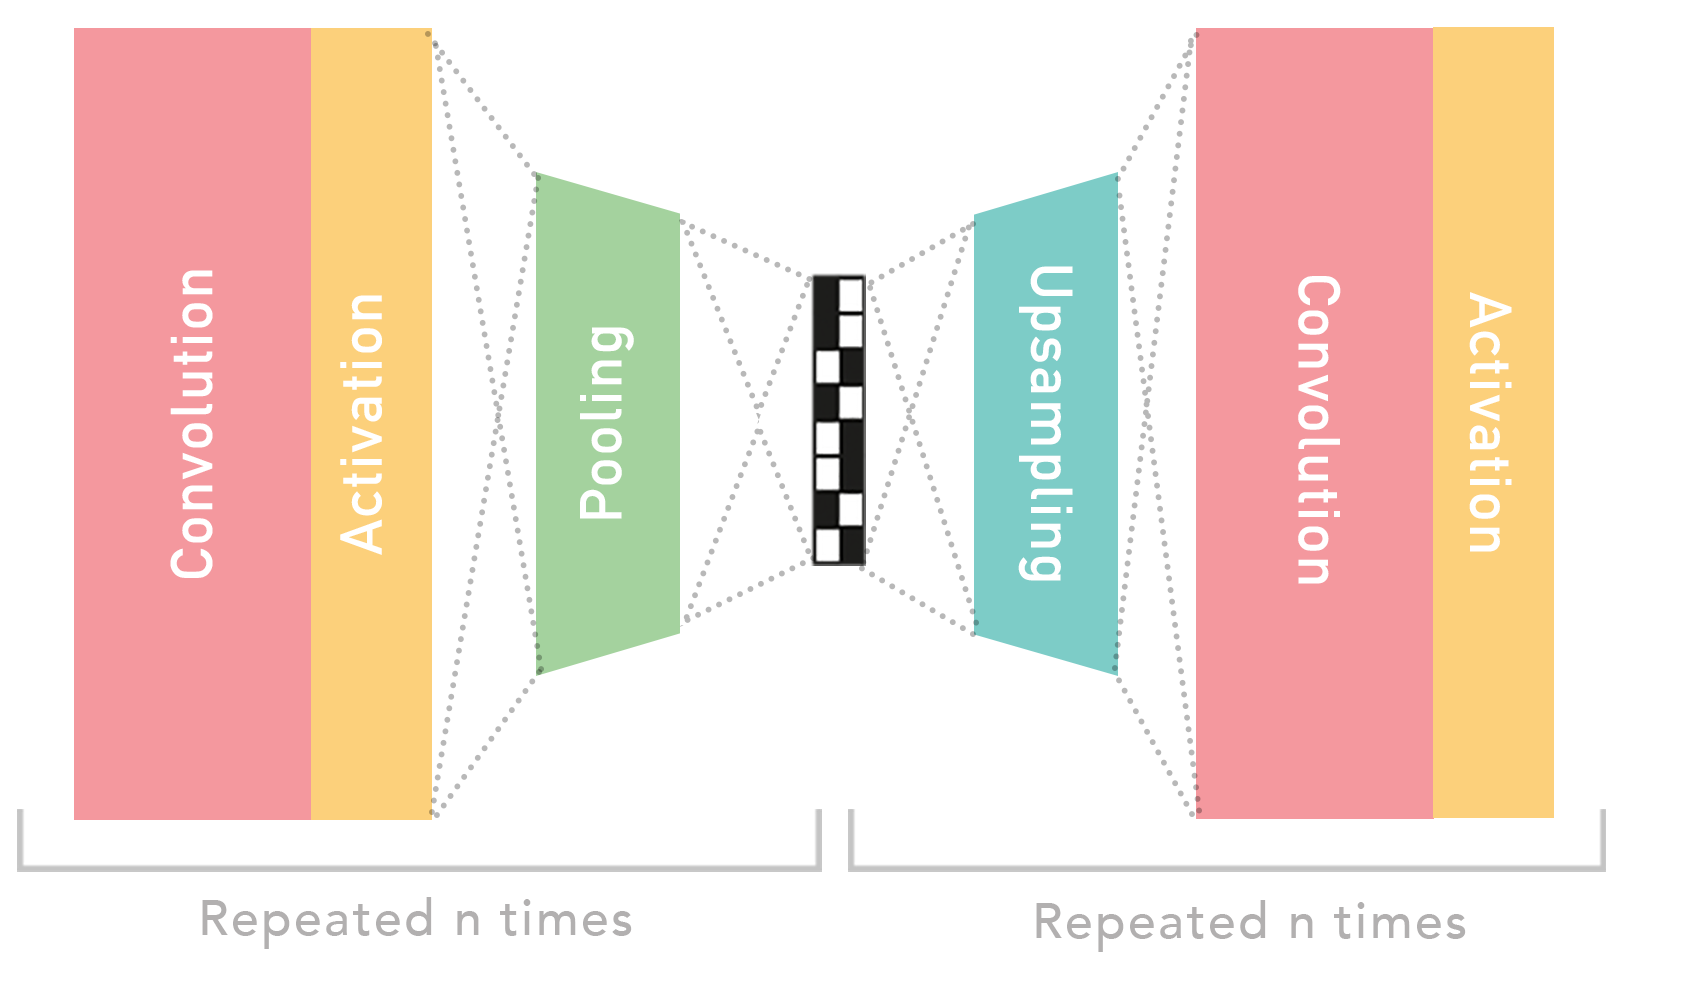
\includegraphics[width=0.6\textwidth]{dissertation/figures/autoencoder_repeat_structure.png}
    \caption{Diagram for a typical autoencoder structure. Operations are symmetrical for the input to be reconstructed with the same dimensions at the output.}
    \label{fig:symmstruc}
\end{figure}

\textit{Convolution} refers to the process of taking the weighted sums of neighbouring values. Put another way, convolutional layers can be thought as a window sliding over an image and summing everything within that window. The specific behaviour of a convolution operation is determined by the filter it uses. Each element in the window will be multiplied by the corresponding element of the filter. We can specify both how big the filter should be, as well as how many different filters should be used. If we use 64 filters, we will learn 64 features about the image, but it will also multiply our dimensions by 64. Figure \ref{fig:convolution} illustrates the convolution process.

\begin{figure}[h]
    \centering
    \missingfigure[]{}
    \caption{Step-by-step illustration of a simple convolution operation on a 4x4 image with a 2x2 kernel. Adapted from Dumoulin and Visin, 2016 (\cite{https://github.com/vdumoulin/conv_arithmetic})}
    \label{fig:convolution}
\end{figure}

\textit{Activation functions} define whether or not each element in the output of the convolutional layer (in this case) should be set to `on' or `off' i.e. whether it should be activated. The purpose of an activation function is to only keep elements of the hidden layers' outputs if it seems to be contributing to the learning of the model.

\textit{Pooling layers} will downsample an image by passing a window over an image and selecting a set value from that window as the one to keep. There are two main types of pooling operations commonly used: average pooling and maximum pooling. In average pooling, the mean value of a window will be chosen as output. In maximum pooling, the maximum value of a window will be chosen. Their counterpart are \textit{upsampling layers} which will resize an image to the right dimensions for a convolutional operation to be applied to it. An illustration of the how these layers function is provided in Figure \ref{fig:sampling}. Using a combination of upsampling and convolutional layers is an alternative to using deconvolution layers which have the drawback of creating checkerboard artifacts (Odena et al., 2016 \cite{https://distill.pub/2016/deconv-checkerboard/})

%https://www.oreilly.com/library/view/deep-learning-for/9781788295628/467cf02b-dc52-49c5-9289-b2721f6758da.xhtml
% http://cs231n.github.io/convolutional-networks/#pool
\begin{figure}[h]
    \centering
    \missingfigure[]{}
    \caption{Left: maximum pooling of 2x2 with stride of 2 applied to a 4x4 image. The image is reduced by a factor of 2. Right: upsampling Right: upsampling of 2x2 with stride of 2 applied to a 2x2 image. The image is augmented by a factor of 2. Adapted from (\cite{http://cs231n.github.io/convolutional-networks/#conv})}
    \label{fig:sampling}
\end{figure}

Throughout the development of the autoencoder, the aim was to maximise the reduction of dimensionality while maintaining a satisfactory reconstructed image. A trade-off had to be done. Size of the coded representation was mainly impacted by the number of hidden layers and size of the convolution and pooling filters. Quality of the reconstructed image could be improved with larger features being used in the convolutional layers and smaller filters.

\bigskip
\subsubsection{Implementation choices}
\hfill
\hfill

Knowing this, the structure of the autoencoder was tuned by trial and error and literature review of existing neural networks for other applications.

In order to avoid losing too much detail in the reconstructed image, we only used 3x3 filters in convolution layers and pooling was done by a factor of 2. Moreover, we kept the number of filters in convolution layers relatively high so as not to lose too much detail in the images. Our structure also used decreasing filter size instead of increasing filter size. Even though increasing filter size showed slight improvements in reconstruction, they are minimal, and having bigger filters towards the bottleneck layer generated bigger coded dimensions. We also decided to replace the pooling operation in the last layer before the bottleneck by a strided convolution layer, because our experiments showed that the colours in the reconstructed image seemed slightly brighter when using striding over pooling (see Figure \ref{}).

In the hidden layers, the choice of activation function was a variant of the Rectified Linear Unit (ReLU), Parametric Rectified Linear Unit (PReLU). ReLU simply returns 0 if the weight unit in the output of a layer is less than 0, or the actual weight if it is bigger than 0. It has become popular because it has been shown to outperform the conventional sigmoid function (\cite{V. Nair and G. E. Hinton. Rectified linear units improve
restricted boltzmann machines. In ICML, pages 807–814,
2010.}, \cite{X. Glorot, A. Bordes, and Y. Bengio. Deep sparse rectifier
networks. In Proceedings of the 14th International Conference on Artificial Intelligence and Statistics, pages 315–323,
2011.}), as well as helping with faster training convergence (\cite{A. Krizhevsky, I. Sutskever, and G. Hinton. Imagenet classification with deep convolutional neural networks. In NIPS,
2012.}). PReLU differs from ReLU by having a small slope for negative values which means it does not map all negative values to 0. This slope is made a learning parameter and is determined by the neural network during training. Figure \ref{relu_prelu} illustrates the difference between the two. He et al., 2015 (\cite{https://arxiv.org/pdf/1502.01852.pdf}) showed that PReLU can improve model fitting for image classification applications. Reconstruction difference using PReLU over ReLU in our network is shown in Figure \ref{}.

\begin{figure}[h]
    \centering
    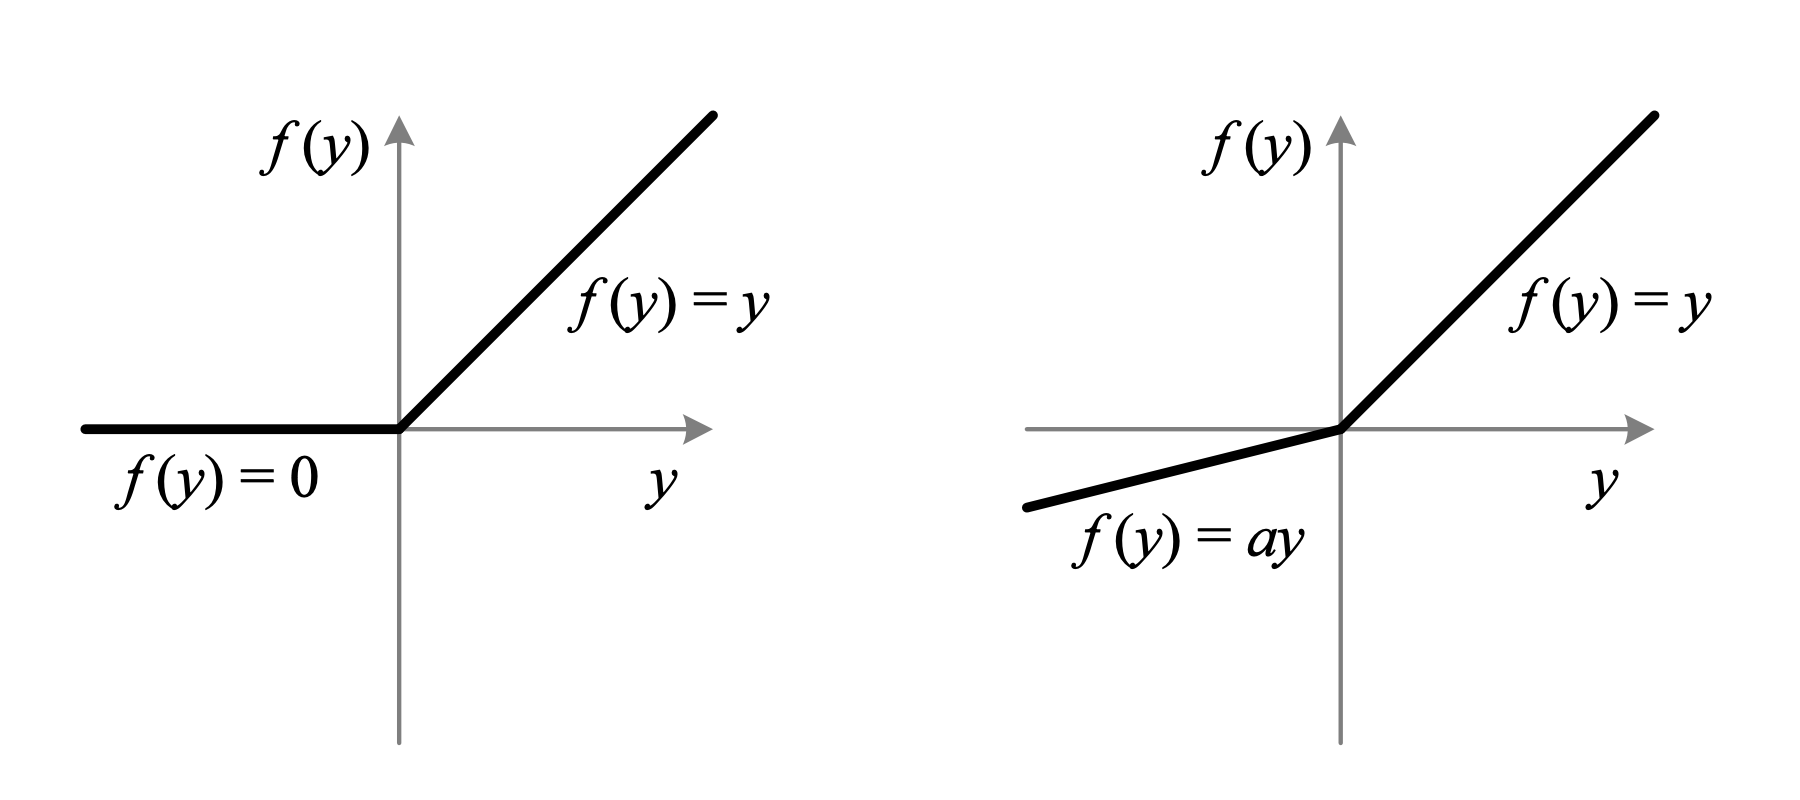
\includegraphics[width=.6\textwidth]{dissertation/figures/relu_prelu.png}
    \caption{[TODO improve] ReLU (left) vs. PReLU (right). The negative part of the PReLU function is variable and a parameter to be learned. Source: He et al., 2015}
    \label{fig:relu_prelu}
\end{figure}

The activation function at the output of the network was the logistic sigmoid activation function, as we needed to restrict output to the [0, 1] range of our image pixels. Figure \ref{fig:sigmoid} illustrates this activation function.

\begin{figure}[h]
    \centering
    \missingfigure[]{Graph showing the logistic sigmoid function slope as well as the equation.}
    \caption{[TODO caption] Logistic sigmoid function.}
    \label{fig:sigmoid}
\end{figure}

Our final autoencoder structure reduced dimensions by a factor of 2 a total of 5 times, resulting in a ten-fold reduction of dimensions on the original 110,592 pixels. The final coded dimensions were of 1,152. Figure \ref{diff_reconstructions} illustrates how the autoencoder reconstructed an input image depending on number of pooling operations. We traded-off some reconstruction quality in order to obtain a smaller coded dimension in the hope that it would help high-dimensional visualisation algorithms perform better, as well as be a better starting block for a regression model.

\begin{figure}[h]
    \centering
    \missingfigure[]{Show reconstruction performance for 3 hidden layers, 4 layers, 5 layers.}
    \caption{Reconstructed images by the autoencoder according to the size of the coded layer. Left shows the input image, and right shows the output image.}
    \label{fig:diff_reconstructions}
\end{figure}

The autoencoder was training with binary cross-entropy as a loss function, as we are aiming to minimise the difference between two distributions: the input, and the reconstructed output. The final structure of the autoencoder is shown below in Figure \ref{fig:autoencoder_details}. Keras code for building the model is available in Listing \ref{lst:autoencoder}.

\begin{figure}[h]
    \centering
    \missingfigure[]{Detailed summary graph of the autoencoder model}
    \caption{[TODO caption]}
    \label{fig:autoencoder_details}
\end{figure}

\subsection{Deep regression}

The regression model was built on the encoder part of the autoencoder. We wanted to use the dimensionality reduction capacities of the encoder layers to evaluate whether interaction could be quantified from an image's feature vector.

The structure of the regression model was kept simple. Research reviewing existing general-purpose neural networks such as VGG-16 showed that adequate tuning of these models obtained results close to `state-of-the-art' without having to resort to more complicated structures. We did not reuse such a general purpose model but the convolutional part of the VGG-16 network is similar to the decoder part of our autoencoder, using 5 combinations of convolutions and pooling operations (Simonyan and Zisserman, 2015). These operations are followed by a small number of fully-connected layers. Hence, we decided to follow this template and not make our regression structure overly complex.

The encoder model was extracted from the autoencoder with the bottleneck layer flattened. This encoder model was then extended with two fully connected layers separated by a dropout layer. Dropout has shown to make models more robust and prevent overfitting (Hinton et al., 2012). The final regression predictions were outputted with a fully connected layer of size 1, activated by a linear function.

The choice of the linear function was justified by the following. The input to the regression model was 192x192x3 images accompanied with labels in the range [0, 100] representing a percentage of overlap between two groups of cells. As such, we want the output activation function to be limited to [0, 100]. Both softplus and linear activations were candidates. The linear activation had to be used with a non-negative kernel constraint, as overlap percentage cannot be negative but the linear function normally allows for negative values. The softplus activation function outputs values in the range [0, $+\infty$]. Performance in terms of training loss was similar, however the linear function performed overall better. Furthermore, softplus does not map an input to itself (shown in Figure \ref{}) and is harder to differentiate compared to the linear function, which would make training slower.

\begin{figure}[h]
    \centering
    \missingfigure[]{Graphs comparing the linear and softplus function.}
    \caption{[TODO caption] Linear function (left) vs. softplus function (right).}
    \label{fig:sigmoid}
\end{figure}

The regression model was trained with mean-squared-error loss, which calculates the difference between the predictions of the model and the truth values of the labels. The final structure of the deep regression model is shown below in Figure \ref{fig:regression_details}. Keras code for building the model is available in Listing \ref{lst:regression}.

\begin{figure}[h]
    \centering
    \missingfigure[]{Detailed summary graph of the regression model}
    \caption{[TODO caption]}
    \label{fig:regression_details}
\end{figure}
